\chapter{Experiments And Results}\label{sec:odometry-experiments-and-results}
	
%\section{Experiments and Results}
% Ablation studies
% Problem with "global" pose -> incremental pose
% Training
%	- Different learning rate for pretrained flownet
%	- Dropout Regularization
	This section presents all experiments conducted on the deep learning model described above.
	The results shown here give useful insights that supplement the work of \cite{wang2017deepvo}.
	
	\section{Dataset Size and Dropout}
		We start by training the proposed model on the KITTI dataset on small subsequences of 25 frames. 
		Initially, the sequences are divided without overlap, that is, each video frame is part of exactly one subsequence.
		In addition, to simulate a dataset with more subsequences, the overlap is set to 20 frames (80\%). 
		This means that for each subsequence there is another that differs by 5 frames.
		Table~\ref{tbl:kitti-overlap-and-dropout} compares the test error for models trained with and without overlap.
		\begin{table}[tb]
			\small
			\begin{center}
				\begin{tabular}{|c|c|c||c|c|c|}
					\hline
					Length 	& Overlap 	& Dropout	& Total 	& Rotation	& Translation	\\ \hline
					25		& 0			& 0			& 19.0293	& 0.4981	& 18.5312		\\ \hline
					25		& 20		& 0			& 16.5471	& 0.3913	& 16.1558		\\ \hline
					100		& 20		& 0			& 529.9459	& 39.8967	& 490.0493		\\ \hline
					100		& 80		& 0			& 313.1278	& 47.8437	& 265.2841		\\ \hline
					100 	& 5			& 0.5		& 376.7666	& 43.1578	& 333.6088		\\ \hline
				\end{tabular}
			\end{center}
			\caption[Experiments on KITTI: Overlap and dropout]
					{Experiments on KITTI: Overlap and dropout. 
				 Shown is the test error on sequence 10 for different overlap and dropout during training.
				 Each model was trained with default parameters for 100 epochs.
				 \todo{also include growing sequence?}
				 \label{tbl:kitti-overlap-and-dropout}}
		\end{table}
		After the same number of epochs, the test error is about 13\% lower for the model trained on overlapping sequences with a decrease of 21\% for rotation and 12\% for translation.
		The same experiment is repeated by training on sequences of 100 frames with overlap 20 vs. overlap 80. 
		% Total error decreases by about 40\%.
		The translation error decreases by almost 46\%, however, the rotation loss increases.
		A similar observation can be made when using dropout on the LSTM output (before the fully-connected layer), as seen in the last row of table~\ref{tbl:kitti-overlap-and-dropout}.
		From these experiments, we can conclude that sequence overlap and dropout have a positive impact on the generalization of translation estimates.
		
		
	
	\section{The Problem on Long Sequences}
	
	
		\begin{table}[tb]
			\small
			\begin{center}
				\begin{tabular}{|c|c||c|c|c|}
					\hline
					Training length & Test length 	& Total 	& Rotation	& Translation	\\ \hline
					25				& 25			& 16.5471	& 0.3913	& 16.1558		\\ \hline
					25				& 100			& 1060.7528	& 37.6196	& 1023.1332		\\ \hline
					100				& 100			& 529.9459	& 39.8967	& 490.0493		\\ \hline
				\end{tabular}
			\end{center}
			\caption[Experiments on KITTI: Testing on longer sequences]
					{Experiments on KITTI: Testing on longer sequences. 
				 When testing on longer sequences, the error becomes extremely high compared to the model trained on 100 frames.
				 \label{tbl:kitti-testing-on-longer-sequences}}
		\end{table}

		\begin{figure}
			\centering
			\begin{subfigure}[b]{0.5\linewidth}
				\centering
				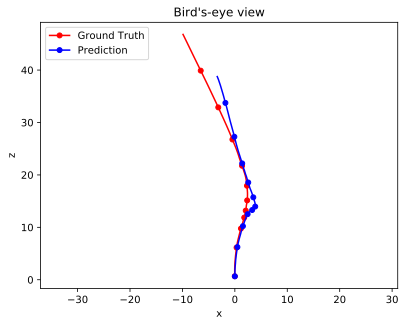
\includegraphics[width=\linewidth]{Experiments/trained-on-25-frames}
				\caption{
					\label{fig:0}
				}
			\end{subfigure}%
			\begin{subfigure}[b]{0.5\linewidth}
				\centering
				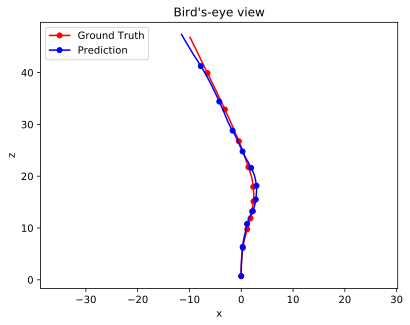
\includegraphics[width=\linewidth]{Experiments/trained-on-100-frames}
				\caption{
					\label{fig:1}
				}
			\end{subfigure}%
			\caption[Training and testing on different sequence length]
					{Training and testing on different sequence length. 
				 Two models tested on a KITTI subsequence of 100 frames and trained on sequences of (a) 25 frames and (b) 100 frames. 
				 The markers in the plot are shown every ten frames.
				 The scale of the axes is in meters.
				 \label{fig:kitti-testing-on-longer-sequences}}
		\end{figure}


	\section{Training with Incremental Poses}

		\begin{figure}
			\centering
			\begin{subfigure}[b]{\linewidth}
				\centering
				\includegraphics[width=0.45\linewidth]{example-image-a}
				\includegraphics[width=0.45\linewidth]{example-image-a}
				\caption{
					Long, curve
					\label{fig:0}
				}
			\end{subfigure}%
			\\
			\begin{subfigure}[b]{\linewidth}
				\centering
				\includegraphics[width=0.45\linewidth]{example-image-b}
				\includegraphics[width=0.45\linewidth]{example-image-b}
				\caption{
					Short
					\label{fig:0}
				}
			\end{subfigure}%
			\\
			\begin{subfigure}[b]{\linewidth}
				\centering
				\includegraphics[width=0.45\linewidth]{example-image-c}
				\includegraphics[width=0.45\linewidth]{example-image-c}
				\caption{
					\label{fig:0}
				}
			\end{subfigure}%
			\caption[Qualitative results for motion estimation on KITTI]
					{Qualitative results for motion estimation on KITTI.
				 Left column: Visualization of the estimated and true path.
				 Right column: Plot of each coordinate axis.
				 Markers are shown for every \todo{xx} frames.
					\label{fig:0}}
		\end{figure}


		\begin{figure}
			\centering
			\begin{subfigure}[b]{\linewidth}
				\centering
				\includegraphics[width=0.45\linewidth]{example-image-a}
				\includegraphics[width=0.45\linewidth]{example-image-a}
				\caption{
					Long, curve
					\label{fig:0}
				}
			\end{subfigure}%
			\\
			\begin{subfigure}[b]{\linewidth}
				\centering
				\includegraphics[width=0.45\linewidth]{example-image-b}
				\includegraphics[width=0.45\linewidth]{example-image-b}
				\caption{
					Short
					\label{fig:0}
				}
			\end{subfigure}%
			\\
			\begin{subfigure}[b]{\linewidth}
				\centering
				\includegraphics[width=0.45\linewidth]{example-image-c}
				\includegraphics[width=0.45\linewidth]{example-image-c}
				\caption{
					\label{fig:0}
				}
			\end{subfigure}%
			\caption[Qualitative results for motion estimation on VIPER]
					{Qualitative results for motion estimation on VIPER.
				 \label{fig:0}}
		\end{figure}